\documentclass[12pt]{article}
\usepackage{fullpage,enumitem,amsmath,amssymb,graphicx}
\usepackage{listings}
\usepackage{tikz}
\usepackage{hyperref}
\usepackage{multirow}

\begin{document}

\begin{center}
{\Large CS 228 Winter 2018 Homework 3}

\begin{tabular}{rl}
SUNet ID: & 05794739 \\
Name: & Luis Perez \\
Collaborators: & \\
Late Days: & 0
\end{tabular}
\end{center}

By turning in this assignment, I agree by the Stanford honor code and declare
that all of this is my own work.

\section*{Problem 1}
It is actually relatively straight-forward to come up with such an example. Consider the Bayes Net in Figure \ref{fig:bayes_mmap_map_diff}, which consits of two binary variables $X_1, X_2$ where $X_1 \to X_2$.

\begin{figure}[!h]
	\centering
	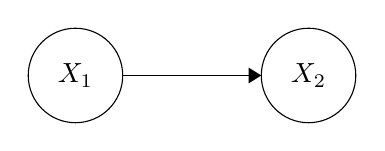
\begin{tikzpicture}[scale=0.2]
		\tikzstyle{every node}+=[inner sep=0pt]
		\draw [black] (27.3,-19) circle (3);
		\draw (27.3,-19) node {$X_1$};
		\draw [black] (42.1,-19) circle (3);
		\draw (42.1,-19) node {$X_2$};
		\draw [black] (30.3,-19) -- (39.1,-19);
		\fill [black] (39.1,-19) -- (38.3,-18.5) -- (38.3,-19.5);
	\end{tikzpicture}
	\caption{Figure of a Simple Bayes Net where marginal MAP assignments for $X_2$ does not match the MPE assigments of $X_2$.}
	\label{fig:bayes_mmap_map_diff}
\end{figure}

Note that the above Bayes net is fully-connected, so it can represent any joint distribution over $X_1, X_2$. As such, let us consider an arbitrary joint distribution, as show in Table \ref{table:arbitrary_joint}.

\begin{table}[!h]
\centering
\begin{tabular}{|c|c|c|c|}
\hline
\multirow{2}{*}{}     & \multicolumn{3}{c|}{x\_1}            \\ \cline{2-4} 
                      &            & \textbf{1} & \textbf{0} \\ \hline
\multirow{2}{*}{x\_2} & \textbf{1} & a          & b          \\ \cline{2-4} 
                      & \textbf{0} & c          & 1-(a+b+c)  \\ \hline
\end{tabular}
\caption{Arbitrary Joint Distribution over Two Binary Variables}
\label{table:arbitrary_joint}
\end{table}
We enforce that this is a valid distribution by making sure all entries are non-negative and making sure the entries sum to one.

Now let us suppose that our evidence is none (ie, $E = \emptyset$). We first recall that we can calculate the MAP or MPE as follows:
\begin{align*}
(x_1, x_2) = \arg\max_{x_1,x_2} p(x_1, x_2 \mid E) = \arg\max_{x_1,x_2} p(x_1, x_2) = \arg\max_{x_1,x_2} p(x_2\mid x_1)p(x_1)
\end{align*}
and that we calculate the marginal MAP for the variable $X_2$ given $E$ as:
\begin{align*}
x_2 = \arg\max_{x_2} \sum_{x_1} p(x_1, x_2 \mid E) = \arg\max_{x_2} \sum_{x_1} p(x_1, x_2) = \arg\max_{x_2}\sum_{x_1} p(x_2\mid x_1)p(x_1)
\end{align*}

What the problem asks us to do is to find an joint distribution such that the $x_2$ found by the first equation is different from the $x_2$ in the second equalition. WLOG, suppose we want the first equation to give us $x_2 = 1$ and the second to give use $x_2 = 0$. In that case, the MMAP imposes the constraint:
$$
c + 1-(a+b+c) > a + b \implies a + b < \frac{1}{2}
$$
The MAP or MPE constraint is simply, WLOG, that $a > c$ and $a > 1 - (a + b + c)$. Solving for $c$, we have the constraint that $1 - 2a - b < c < a$.

There are many solutions to these constraints, but for concreteness, let us simply take $b = 0$, $a = \frac{4}{10}$, and $c = \frac{3}{10}$ which we can check satisfies all of the above constraints. This gives us the joint distributions as in Table \ref{table:constraint_joint_solution}:
\begin{table}[!h]
\centering
\begin{tabular}{|c|c|c|c|}
\hline
\multirow{2}{*}{}     & \multicolumn{3}{c|}{x\_1}            \\ \cline{2-4} 
                      &            & \textbf{1} & \textbf{0} \\ \hline
\multirow{2}{*}{x\_2} & \textbf{1} & $\frac{4}{10}$          & $0$          \\ \cline{2-4} 
                      & \textbf{0} & $\frac{3}{10}$          & $\frac{3}{10}$  \\ \hline
\end{tabular}
\caption{One Possible Solution to our Constraints}
\label{table:constraint_joint_solution}
\end{table}

Alternatively, we can specify the conditional probabilities directly. Consider the following probability distributions for the above Bayes Net, as in Table:
\begin{table}[!h]
\centering
\begin{tabular}{|c|c|}
\hline
$P(X_1 = x_1)$ & $x_1$ \\ \hline
$\frac{7}{10}$            & 1    \\ \hline
$\frac{3}{10}$            & 0    \\ \hline
\end{tabular}
\quad
\begin{tabular}{|c|c|c|}
\hline
$P(X_2 = x_2 \mid X_1 = x_1)$ & $x_2$ & $x_1$ \\ \hline
$\frac{4}{7}$                          & 1    & 1    \\ \hline
$\frac{3}{7}$                          & 0    & 1    \\ \hline
0                          & 1    & 0    \\ \hline
$1$                          & 0    & 0    \\ \hline
\end{tabular}
\caption{Conditional Distributions of our Joint Example}
\label{table:conditional_distributions}
\end{table}

In this case, we note that the MLE is given by $x_1 = 1, x_2 = 1$ (since this is the max value over the joint). However, if we consider the MMAP for $x_2$, we have $p(x_2 = 0) = \frac{6}{10}$ and $p(x_2 = 1) = \frac{4}{10}$, so the MMAP for $X_2$ is actually $x_2 = 0$.

In this case, we note that the maximum is actually achieved for $x_2 = 1$ as the value of $p(0,1) + p(1,1) = 0.36 + 0.09 = 0.45$ as opposed to $x_2 = 0$ which has value of $p(0,0) + p(1,0) = 0.01 + 0.54$

\pagebreak
\section*{Problem 2}

\begin{enumerate}[label=(\alph*)]
  \item The algorithm is simply the variable elemination algorithm presented in class repeated for each pair of $X_i, X_j$. For each pair, we know that Variable Elimination will take $O(nd^3)$ by the results derived in class, so our algorithms running time is $O(n^3d^3)$. However, we present the algorithm and proof of its running time in detail here, for completeness. 

  First we note that the joint distribution is given by:
  $$
  	P(X_1, \cdots, X_n) = \frac{1}{Z}\prod_{i=1}^{n-1} \phi(X_i, X_{i+1})
  $$
  where $Z$ is the normalization constant. Note that $P(X_i, X_j) = P(X_j, X_i)$, so WLOG of assume $i < j$. We have $O(n^2)$ such pairs. Now, for a single pair, we use the Variable Elimation algorithm to compute $P(X_i, X_j)$. Mathematically, we wish to compute:
  \begin{align*}
  	P(X_i, X_j) &= \sum_{x_k \forall k \neq i,j} P(X_1, \cdots X_n) \\
  	&= \frac{1}{Z} \sum_{x_k \forall k \neq i,j} \prod_{\ell = 1}^{n-1}\phi(X_{\ell}, X_{\ell+1}) \\
  	&=\frac{1}{Z} \sum_{x_1} \phi(X_1, X_2) \\
  	&\cdots \sum_{x_{i-1}}\phi(X_{i-2}, X_{i-1})\phi(X_{i-1}, X_{i}) \sum_{x_{i+1}} \phi(X_i, X_{i+1}) \\
  	&\cdots \sum_{x_{j-1}}\phi(X_{j-2}, X_{j-1})\phi(X_{j-1}, X_{j}) \sum_{x_{j+1}} \phi(X_j, X_{j+1}) \\
  	&\cdots \sum_{x_n} \phi(X_{n-1}, X_n)
  \end{align*}
  The above is presented in the full generality. Note that our variable elimination algorithm can work on the above from right to left, considering only the pseudo-factors containing $X_z$. In detail:
  \begin{enumerate}
  	\item We begin with $z=n$ where we consider the factor $\phi(X_{n-1}, X_n)$ and marginalize out $X_n$, giving us a pseudo factor $\Phi(X_{n-1})$.
  	\item We can merge with $\phi(X_{n-2}, X_{n-1})$ to form the pseudo-factor $\Phi(X_{n-2}, X_{n-1})$. Note that this process takes $O(d^2)$ time.
  	\item We will continue in this fashion until we form the pseudo-factor $\Phi(X_{j-1}, X_j)$, at which point we don't marginalize out $X_j$ but instead marginalize out $X_{j-1}$. The pseudo-factors following this are always of the form $\Phi(X_k, X_j)$ for $k < j$ where at each step we marginalize out $X_k$, each step taking $O(d^2)$ time. 
  	\item Eventually, we will form the pseudo-factor $\Phi(X_i,X_j)$, at which point we do \textbf{not} marginalize $X_i$ and instead continue to form the larger pseudo factor $\Phi(X_{i-1}, X_i, X_j)$, where we now marginalize $X_{i-1}$. Note that the running time for this part is now $O(d^3)$. 
  	\item We continue as such with pseudo-factors $\Phi(X_k, X_i, X_j)$ for $k < i$ until the pseudo factor $\Phi(X_1, X_i, X_j)$, which after marginalization, becomes simply $\Phi(X_i, X_j)$.
  	\item At this point, we have all unnormalized values of $\Phi(X_i, X_j)$, so we simply normalize with by $Z = \sum_{i,j} \Phi(X_i, X_j)$ such that we have a valid joint probability distribution.
  \end{enumerate}
  We must repeat the above for $O(n^2)$ such $X_i,X_j$ pairs. Note that the running time for each pair is essentially $O(id^3 + (n-i)d^2)$. We note that approximately $\frac{1}{4}$ of all pairs have $i > \frac{n}{2}$, and for these $\frac{n^2}{4}$ pairs the running time of each is therefore $O(nd^3)$. As such, the running time of the full algorithm is $O(n^3d^3)$, as expected.

  \item This is purely an exercise in notation. For simplicity, we define the following function:
  $$
  	\Gamma_{y,z} = \sum_{X_m \forall y \leq m \leq z } \prod_{k=y}^z \phi(X_{k-1}, X_{k})
  $$
  where we know that
  $$
  	P(X_1, \cdots, X_n) = \frac{1}{Z} \prod_{i=2}^{n} \phi(X_{i-1}, X_i)
  $$
  The above function simply defines the partially pushed sum into the factors of the probability distribution. WIth the above defined, we can proceed to prove the given identity. We begin with the RHS and simplify to the LHS.
  \begin{align*}
  	&\sum_{X_{j-1}} P(X_i, X_{j-1})P(X_j \mid X_{j-1}) \\
  	&= \sum_{X_{j-1}} \frac{P(X_{i}, X_{j-1})P(X_{j-1}, X_j)}{P(X_{j-1})} \tag{Bayes Rule} \\
  	&= \sum_{X_{j-1}} \frac{\left[\frac{1}{Z} \Gamma_{1, i-1} \phi(X_{i-1}, X_{i}) \Gamma_{i + 1, j-2} \phi(X_{j-2}, X_{j-1}) \Gamma_{j, n}\right]\left[\frac{1}{Z}\Gamma_{1, j-2} \phi(X_{j-2}, X_{j-1})\phi(X_{j-1}, X_j)\Gamma_{j+1, n} \right] }{\frac{1}{Z}\Gamma_{1, j-2} \phi(X_{j-2}, X_{j-1}) \Gamma_{j, n})} \tag{Pushing Sums In} \\
  	&= \sum_{X_{j-1}} \frac{1}{Z}\Gamma_{1, i-1}\phi(X_{i-1}, X_i)\Gamma_{i+1, j-2}\phi(X_{j-2}, X_{j-1})\phi(X_{j-1},X_j)\Gamma_{j+1, n} \tag{Cancelling Like Terms} \\
  	&=  \frac{1}{Z}\Gamma_{1, i-1}\phi(X_{i-1}, X_i)\Gamma_{i+1, j-1}\phi(X_{j-1},X_j)\Gamma_{j+1, n} \tag{Pushing outer sum in and simplifying using $\Gamma$} \\
  	&= P(X_i, X_j) \tag{Definition of $\Gamma$ (ie, we're summing the potentials over everything except $X_i, X_j$)}
  \end{align*}
  And we are done in our excercise with notation.
  \item The algorithm is rather straigh-forward and simply an excersice in dynamic programming. I describe it step by step below, and provide arguments for correctness for each step as well as arguments describing the time-complexity of each step.

  \begin{enumerate}
  	\item We begin by computing $P(X_i, X_{i+1})$ for $1 \leq i \leq n$ (ie, we compute the joint probability of all adjacent pairs). We do this directly, by using the algorithm described in Part (a) above. As such, the running time is $O(n^2d^3)$ (since for each $i$, the naive algorithm from (a) takes $O(nd^3)$) and we have $O(n)$ such $i$. 
  	\item We also compute $P(X_i)$ for $1 \leq i \leq n$. We can do this rather efficinetly given $P(X_i, X_{i+1})$ simply by marginalizing out $X_{i+1}$. This process will take $O(d^2)$ time for each $i$ which gives a total running time for this step of $O(nd^2)$.
  	\item For $k \in \{2,\cdots, n-1\}$ processed from smallest to largest, we compute $P(X_i, X_{i+k})$ for all $1 \leq i \leq n$ using the formula from above which simplifies to:
  	$$
  		P(X_i, X_{i+k}) = \sum_{X_{i+k-1}} \frac{P(X_i, X_{i+k-1})P(X_{i+k-2}, X_{i+k-1})}{P(X_{i+k-1})}
  	$$
  	Note that $P(X_{i+k-1})$ and $P(X_{i+k-2}, X_{i+k-1})$ were already computed at the start of the algorithm, and therefore, these operations consists of a simple lookup. Furthermore, note that $P(X_i, X_{i+k-1})$ must have already been computed since this is the same as $P(X_i, X_{i+k'})$ where $k' = k - 1$ and we process the values of $k$ in increasing order. Therefore, this too consists of a simple lookup. As such, the running time of this process for a single value of $k$ and $i$ is $O(d^3)$. Since we need only process $O(n)$ values of $i$ for each of the $O(n)$ values of $k$, the total running time for this step is $O(n^2d^3)$.
  	\item Note that at this point, we have computed $P(X_i,X_j)$ for all values of $i < j$ (and as in (a), the joins are symmetric).
  \end{enumerate}

  As such, we can clearly see from the above that the algorithm runs in $O(n^2d^3)$ which is asymtotically faster than the naive algorithm from (a) which ran in $O(n^3d^3)$.

\end{enumerate}

\pagebreak
\section*{Problem 3}

\begin{enumerate}[label=(\alph*)]
\item We modifiy a factor in some clique $C_i$, which means we modify its clique potential $\phi(C_i)$. If we consider the clique tree as rooted at $C_i$, we can see how this will require that we update all outgoing messages from $i$ to its children (the downward pass from the root), and similarly this will trigger an update for all messages from the children to their children until we reach the leaf nodes. In all, this single-pass will require updating $N-1$ of the messages, specifically updating all $\delta_{p \to c}$ such that $p$ is the parent of $c$ in a tree rooted at $C_i$.
\item In this case, since we are only interested in the marginal of $X_k$, we can compute even fewer message updates. That is to say, we consider the clique tree as if it were rooted at $X_i$, and we iterate through the clique nodes in post order so that we can compute $X_k$ using the messages $\delta_{c \to p}$ where $p$ is the parent of $c$ in the tree rooted at $X_k$. We note that the only messages affected by the change in $C_i$ in this case are the messages sent along the path from $i \to k$. In this worst case, we will need to recompute $N - 1$ messages (if, for example, $i = 1$ and $k=N$ and our tree is linear $C_1 \to \cdots \to C_N$. However, we can see that in most cases, we will need to re-compute less than $N - 1$ message updates since a large portion of our graph will already be computed (for example, supposed we have $i = N - 1$ and $k = N$ for a linear $C_ 1 \to \cdots \to C_{N-1} \to C_{N}$, in which case we'd only need to recompute $\delta{N-1 \to N}$).
\end{enumerate}

\pagebreak
\section*{Problem 4}

\begin{enumerate}[label=(\alph*)]
\item 
	\begin{itemize}
		\item Is $P(x\mid e)$ tractable? No. We cannot compute $P(x \mid e)$ in a tractable way. This is because in order to compute $P(x \mid e)$ we would need to compute $P(e)$, which would require marginalizing out over $X$, which in general, could be intractable (ie, $X$ is a clique).
		\item Can we sample directly from the distribution $P(X \mid e)$. No. We would need to compute $P(X_i \mid e, Pa(X_i)$ for all $X_i$, which in general, would be difficult to do so and intractible.
		\item Can you compute $P(x,e)$ in a tractable way? Yes. This is simply the full joint, which the Bayes net implicitly fully specifies and will therefore consists simply of, at most, a product over $n$ values.
	\end{itemize}
	\item While computing $Q(X \mid E = e)$ is not tractable (even for the given tree network, since computing $Q(E = e)$ is required and this itself might require marginalizing out the root in the case where the root is not in $E$ which would lead to an induced graph with a clique of size $n-1$ meaning that variable elimination would take $O(n^{n-1}$ time). However, we can still sample from $Q(X \mid E = e)$ using the following algorithm:
		\begin{itemize}
			\item The sampling problem becomes tractable because of the structure of the graph. Suppose the graph consists of variables $R, C_1, \cdots, C_n$ with edges $R \to C_i$. Then we are given by the Bayes Net the following CPTs (which are multinomial, and from which we can sample efficiently), $r \sim Q(R)$ and $c_i \sim Q(C_i \mid R = r)$. We further note that $Q(C_1, \cdots, C_n, R) = Q(R)\prod_i Q(C_i \mid R)$.
			\item Consider the simple case where $R \in E$, so we have a known value $R = r$. In this case, we note that $C_i \perp C_j \mid R = r$, so we can simply sample $x_i \sim Q(X_i \mid E = e) = Q(X_i \mid R = r)$ directly from the CPTs provided by the tree bayes net.
			\item We consider the slightly more difficult case where $R \notin E$. In this case, we focus first on sampling a value $r \sim Q(R \mid E)$. The problem is computing the CPT for $Q(R = r \mid E = e)$. However, we note that by Bayes Rule:
			$$
				Q(R = r \mid E=e) \propto \sum_{X \setminus \{R\}} Q(R=r, E=e, X \setminus \{R\})
			$$
			Note that the above is marginalization over only child-nodes, which we can directly perform using the variable elimination algorithm in $O(n^2)$ time due to the graph structure. We need to compute it for all values of $R$, so the running time is tractable $O(|Val(R)|n^2)$. Once we've computed for all values of $R$, we can normalize and obtain the CPT $Q(R = r \mid E = e)$, which is simply a multinomial distributions. We store the CPT $Q(R \mid E = e)$ in this case for future usage.
			\item We then sample $r \sim P(R \mid E=e)$ from above.
			\item Once we have $r$, it again becomes trivial to sample $x_i \sim (X_i \mid E=e, R=r) = Q(X_i \mid R= r)$ since these CPTs are given directly by the Bayes Net. 
			\item Return the sampled values for $X = \{x_i\}$.
		\end{itemize}
	\item We now consider how to compute the weight $w[m]$ given a sample $x[m] \sim Q(X\mid E = e)$. First, let us consider and indicator function $\delta_x(x)$ which is $1$ if $x$ is consistent with $X = x$ and $0$ otherwise. Then we can write:
		\begin{align*}
			P(X = x \mid E = e) &= \frac{P(X = x, E=e)}{P(E=e)} \tag{Bayes Rule} \\
			&= \frac{\sum_{X} \delta_x(x)P(X = x, E=e)}{\sum_{X} P(X= x, E=e)} \tag{Marginalizing over X and using Indicator Function} \\
			&= \frac{\sum_{X} \delta_x(x)P(X = x, E=e)\frac{Q(X=x\mid E =e)}{Q(X = x \mid E = e)}}{\sum_{X} P(X= x, E=e)\frac{Q(X=x\mid E =e)}{Q(X = x \mid E = e)}} \tag{multiplied by $1$ top and bottom} \\
			&= \frac{\sum_{X} \delta_x(x)w[x]Q(X = x \mid E = e)}{\sum_{X} w[x]Q(X = x \mid E = e)} \tag{defined $w[x] = \frac{P(X = x, E =e)}{Q(X = x \mid E = e)}$}\\
			&= \frac{E_{Q(X \mid E = e)}[\delta_x(x)w[x]]}{E_{Q(X \mid E = e)}[w[x]]}
		\end{align*}
		As such, with the above derivation, we can define our weights for our samples as follows:
		$$
			w[m] = \frac{P(X = x[m], E = e)}{Q(X = x[m] \mid E = e)}
		$$
		Note that computing $P(X = x[m], E = e)$ is tractable, since we're simply computing the full joint distribution on $P$ (which is at most $n$ multiplications). We consider how to efficiently compute the denominator $Q(X = x[m] \mid E = e)$. Consider two cases.
		\begin{itemize}
			\item $R \in E$. In this case, we have:
				$$
					Q(X = x \mid E = e) = Q(X = x \mid R) = \prod_{i} Q(X_i = x_i \mid R)
				$$
				which we can compute efficiently and directly given the CPTs from the Bayes Networks.
			\item $R \not in E$. In this case, note that we computed $Q(R \mid E=e)$ and saved the CPT above. Therefore, we have the below, where $\tilde{X}$ is $X$ without $R$:
			\begin{align*}
			Q(X = x \mid E = e) &= Q(\tilde{X} = \tilde{x}, R = r \mid E = e) \\
			&= Q(\tilde{X} = \tilde{x} \mid R = r, E =e )Q(R=r \mid E=e) \\
			&= \prod_{i} Q(\tilde{X_i} = \tilde{x_i} \mid R = r)Q(R = r \mid E = e)
			\end{align*}
			which we can compute efficiently in at most $n$ products.

		\end{itemize}

	\item We now show the form of the final estimator. Instead of computing the expectation over $Q$, we can instead estimate it based on our samples. This gives us:
	\begin{align*}
		P(X = x \mid E = e) &= \frac{E_{Q(X \mid E = e)}[\delta_x(x)w[x]]}{E_{Q(X \mid E = e)}[w[x]]} \tag{Results from (i)} \\
		&\approx \frac{\sum_{i=1}^m \delta_x(x[m]) w[m]}{\sum_{i=1}^m w[m]} \\
		&= \hat{P}(X = x \mid E = e)
	\end{align*}
\end{enumerate}


\pagebreak
\section*{Problem 5}


\begin{enumerate}[label=(\alph*)]
\item We verify with the following codes:
	\begin{itemize}
		\item Invalid: $[0, 1, 1, 0, 1, 0]$ which produces $0.0$
    \item Invalid: $[1, 0, 1, 1, 0, 1]$ which produces $0.0$
    \item Valid: $[1, 0, 1, 1, 1, 1]$ which produces $\sim0.039 > 0.0$
	\end{itemize}
\item See source code.
\item We plot the stimated posterior probabability conditioned on the noisy message. We see this plot in Figure \ref{fig:conditional_probability_message}.

\begin{figure}[!h]
\centering
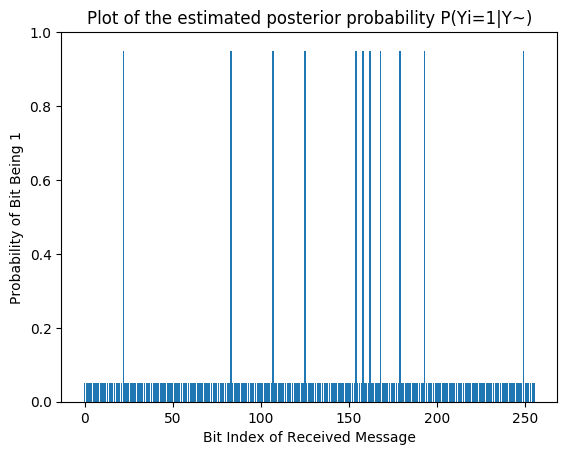
\includegraphics{programming/5c}
\caption{Plot of Each Bit Posterior Probability Conditioned on Evidence}
\label{fig:conditional_probability_message}
\end{figure}

It's not visible, but we essentially have a straight line along $0$. In general, the MMAP does not necessarily give us the right answer. We note that in this case, MMAP does give us the correct answer since it seems that with very high likelihood we set every bit to $0$.

\item We repeat the experiment from above for 10 random channel noise realizations. The results are showing in Figure \ref{fig:low_epsilon}. We note that it seems as if BP is typically reliable, but if enough bits are different, then we will not converge to the true value (for example, we had one trial were $20$ bits were different, and it seems in this case BP did not find the correct marginal probabilites). The reason for this is likely due to the feedback loop which finds a local optimal that is not near the global optimal.

\begin{figure}[!h]
\centering
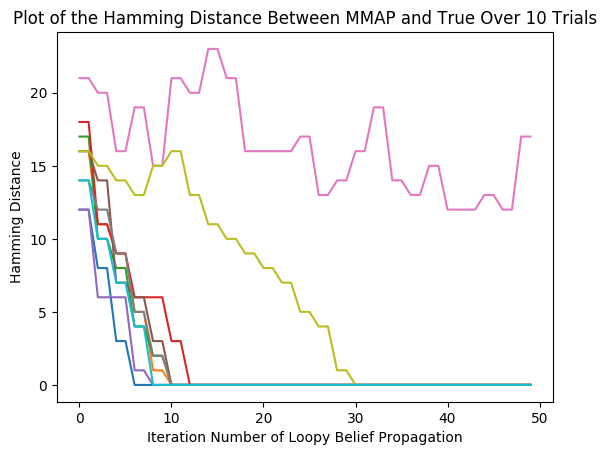
\includegraphics{programming/5d_epsilon=6.png}
\caption{Hamming Distance by Iteration Over 10 Values with $\epsilon = 0.06$.}
\label{fig:low_epsilon}
\end{figure}

\item We repeat the above for higher error probabilities. We note that the higher error probabilities lead to more frequent scenarios where Loopy BP does not perform well. This further supports our hypothesis that the Loopy BP is good at finding solutions when there is not a large amount of noise in the original realization of the value. See Figure \ref{fig:middle_epsilon} and Figure \ref{fig:high_epsilon} for the plots.

\begin{figure}[!h]
\centering
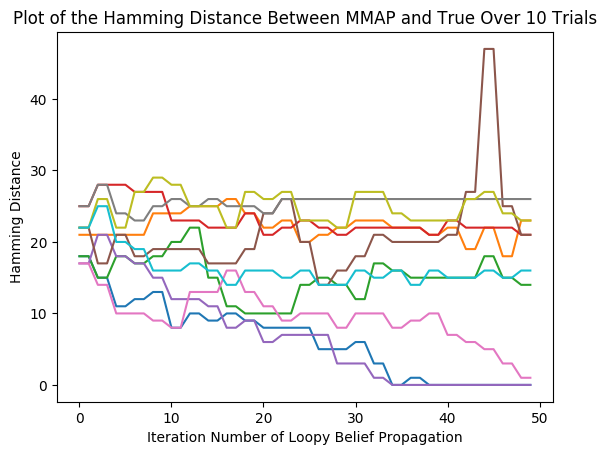
\includegraphics{programming/5d_epsilon=8.png}
\caption{Hamming Distance by Iteration Over 10 Values with $\epsilon = 0.08$.}
\label{fig:middle_epsilon}
\end{figure}

\begin{figure}[!h]
\centering
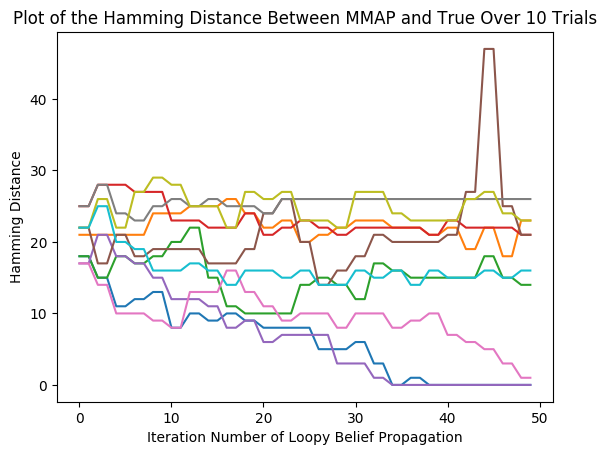
\includegraphics{programming/5d_epsilon=8.png}
\caption{Hamming Distance by Iteration Over 10 Values with $\epsilon = 0.10$.}
\label{fig:high_epsilon}
\end{figure}


\item We use our above decoder to show the result replicating MacKay's Fig 47.5. The results are shown in Figure \ref{fig:imaga_reconstruction}.

\begin{figure}[!h]
\centering
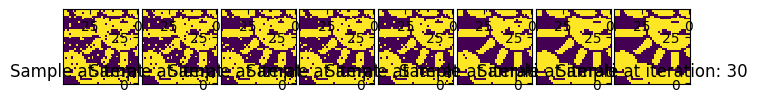
\includegraphics{programming/5fg_error=6.png}
\caption{Image Reconstruction with $\epsilon = 0.06$. We plot for 0, 1, 2, 3, 5, 10, 20 ,and 30 iterations}
\label{fig:imaga_reconstruction}
\end{figure}


\item We repeat the above experiment but with a higher value of $\epsilon=0.10$. We can qualitatively note that our loopy BP algorithm did not converge as well with this amount of noise. See Figure \ref{fig:imaga_reconstruction_2} for reference.

\begin{figure}[!h]
\centering
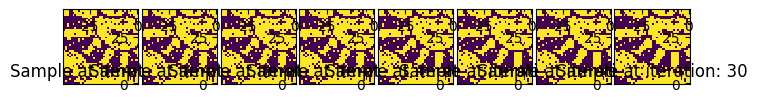
\includegraphics{programming/5fg_error=10.png}
\caption{Image Reconstruction with $\epsilon = 0.10$. We plot for 0, 1, 2, 3, 5, 10, 20 ,and 30 iterations}
\label{fig:imaga_reconstruction_2}
\end{figure}

\end{enumerate}{}


\end{document}
